\chapter{Building Your AI Video Evaluation Framework: A Sora 2 vs.\ Veo 3.1 Case Study}
\label{ch:sora-veo-comparison}
\index{Sora 2!comparison with Veo 3.1}
\index{Veo 3.1!comparison with Sora 2}
\index{platform comparison}
\index{evaluation framework}

\begin{chapterabstract}
As AI video generation platforms evolve at unprecedented speed---with major updates often arriving quarterly---the question ``Which platform is best?'' becomes rapidly obsolete. \textbf{The more valuable skill is knowing \textit{how} to evaluate any AI video tool systematically.} This chapter presents a reusable evaluation framework, demonstrated through a rigorous comparison between OpenAI's Sora 2 and Google's Veo 3.1 (as of late 2025). While specific results will inevitably shift as platforms update, the \textbf{five-dimension testing methodology} and \textbf{evaluation criteria} presented here will remain applicable to Sora 3, Veo 4, and any future platforms. Beyond platform comparison, we introduce the \textit{Five-Dimension Prompt Formula}---a universal methodology for crafting effective Prompts that transcends any single tool.
\end{chapterabstract}

%% ================================================================
\section{Introduction: Why Evaluation Methodology Matters More Than Rankings}
\label{sec:comparison-intro}

\begin{quote}
\textit{\textbf{Timeless Principle:} Platforms will update, interfaces will change, and today's winner may be tomorrow's runner-up. But a systematic approach to evaluating AI capabilities---testing physics, consistency, expression, interaction, and commercial readiness---will serve you for years to come.}
\end{quote}

The AI video generation market has reached an inflection point. While numerous platforms compete for attention---including Runway Gen-3, Kling, and Luma Dream Machine---two systems have emerged as the definitive leaders in 2024--2025: \textbf{OpenAI's Sora 2} and \textbf{Google's Veo 3.1}.

Both platforms represent billions of dollars in research investment and years of foundational model development. Yet they approach video generation with fundamentally different architectural philosophies:

\begin{itemize}
    \item \textbf{Sora 2} leverages OpenAI's expertise in language understanding and multimodal reasoning, excelling at interpreting complex narrative Prompts and generating physically coherent motion sequences.
    \item \textbf{Veo 3.1} builds upon Google DeepMind's research in visual understanding and temporal consistency, prioritizing stable character identity and logical scene coherence.
\end{itemize}

\textbf{Important Note:} The specific results in this chapter reflect platform capabilities as of late 2025. By the time you read this, both platforms may have released significant updates. However, the \textbf{evaluation framework}---the test categories, scoring methodology, and decision criteria---remains fully applicable. Use this chapter not as a definitive ranking, but as a template for conducting your own systematic evaluations.

Rather than relying on marketing claims or cherry-picked demonstrations, this chapter provides transparent, reproducible comparison testing. We use identical Prompts for both platforms and evaluate results across multiple dimensions that matter to professional creators.

\subsection{Testing Methodology}
\label{subsec:testing-methodology}

Our evaluation framework employs five carefully designed test cases, each targeting a specific capability:

\begin{enumerate}
    \item \textbf{Temporal Evolution \& Object Control} --- Can the model maintain logical consistency as objects transform over time?
    \item \textbf{Complex Physics \& Human Dynamics} --- How accurately does the model simulate real-world physics and human biomechanics?
    \item \textbf{Detail Texture \& Emotional Expression} --- Can the model capture subtle expressions and avoid visual artifacts?
    \item \textbf{Hand Details \& Object Interaction} --- How well does the model handle the notoriously difficult task of hand-object manipulation?
    \item \textbf{Commercial Quality \& Audio-Visual Sync} --- Can the output meet professional advertising standards with synchronized sound?
\end{enumerate}

Each test uses the exact same Prompt text for both platforms, with results evaluated by a panel of professional video editors and VFX artists. Let us examine the findings.

%% ================================================================
\section{Test Case 1: Temporal Evolution and Object Control}
\label{sec:test-case-1}

\subsection{Scenario: Home Furnishing Transformation}

This test evaluates how each platform handles long-take temporal consistency---the ability to show a scene transforming over time while maintaining visual coherence.

\begin{promptbox}[Test Prompt: Home Furnishing Scene]
\small
\textbf{Home Furnishing:} Setting up a living room from moving boxes. Base style: ``Realism, natural light, handheld camera texture, 4K.'' Aspect ratio: ``16:9.'' Scene description: ``A newly delivered bare apartment living room with white latex paint walls and light gray floor tiles, large floor-to-ceiling windows. Morning sunlight streams in from outside.'' Camera setting: ``Fixed wide-angle lens position, slightly upward angle, simulating surveillance perspective to completely record the living room's transformation from empty to furnished.'' Core elements: A large cardboard box with delivery labels. Assembly items: chair, monitor, bookshelf, books, pen holder, plants, carpet. Exclusions: no people, no text, no special effects.
\end{promptbox}

\subsection{Evaluation Results}

\paragraph{Veo 3.1 Performance:}
The generated video demonstrated strong frame-to-frame consistency. While objects lacked realistic inertia during movement (appearing to ``slide'' into position rather than being physically placed) and the carpet landing lacked soft material physics, the overall logical progression from empty room to furnished space was successfully achieved. The transformation sequence maintained temporal coherence throughout the clip.

\paragraph{Sora 2 Performance:}
The physics simulation exhibited significant breakdown. Visible frame jumping and flickering artifacts disrupted the viewing experience. Most critically, the ``assembly'' process lacked continuity---objects appeared and disappeared inconsistently rather than following a logical unpacking sequence.

\begin{resultbox}[Test Case 1 Winner: Veo 3.1]
\textbf{Conclusion:} For long-take object evolution and instruction consistency, Veo 3.1 currently delivers superior results. Its architecture prioritizes temporal stability over physics simulation fidelity.
\end{resultbox}

%% ================================================================
\section{Test Case 2: Complex Physics and Human Dynamics}
\label{sec:test-case-2}

\subsection{Scenario: Skateboard Trick Performance}

This test pushes both platforms to their limits with high-speed human motion, complex biomechanics, and real-world physics simulation---one of the most challenging domains for generative video.

\begin{promptbox}[Test Prompt: Skateboard Trick]
\small
\textbf{Skateboard Trick:} Performing a kickflip on a bench at an urban skate park. Dynamic camera follows the entire action. Accompanied by sounds of wheel friction, board flipping, and landing. Afternoon sunlight casts long shadows.
\end{promptbox}

\subsection{Evaluation Results}

\paragraph{Veo 3.1 Performance:}
While the overall motion sequence was complete, the physics simulation revealed significant inaccuracies. During the kickflip rotation, the skateboard appeared magnetically ``attached'' to the skater's feet, lacking realistic gravitational separation. The landing exhibited an overly soft, dampened quality inconsistent with actual skateboard physics.

\paragraph{Sora 2 Performance:}
The results were remarkably impressive. Sora 2 demonstrated sophisticated physics understanding, generating not only the successful trick execution but also realistic failure scenarios---including authentic stumbling, balance recovery attempts, and natural fall dynamics. The skateboard exhibited proper independent motion during the flip phase with zero ``floating'' artifacts. The simulation adhered convincingly to real-world physical laws.

\begin{resultbox}[Test Case 2 Winner: Sora 2]
\textbf{Conclusion:} For complex human biomechanics and high-speed physical motion, Sora 2's physics engine demonstrates clear superiority. Its world model appears to have internalized fundamental physical principles rather than merely pattern-matching visual appearances.
\end{resultbox}

%% ================================================================
\section{Test Case 3: Detail Texture and Emotional Expression}
\label{sec:test-case-3}

\subsection{Scenario: Humorous Living Room Scene}

This test evaluates the platforms' ability to capture subtle emotional expression, maintain logical coherence in whimsical scenarios, and avoid the ``AI hallucination'' artifacts that often plague generative models.

\begin{promptbox}[Test Prompt: Humorous Cat Scene]
\small
\textbf{Humorous Scene:} A humorous living room scene. A lazy, fluffy cat lounges on the sofa, holding a beer mug and a cigarette with its paws. The cat looks both relaxed and guilty. Suddenly, the front door opens and the owner walks in. The cat spills a bit of beer, drops the cigarette, then freezes with wide eyes, displaying an awkward ``caught in the act'' expression... (Emphasize photorealistic quality)
\end{promptbox}

\subsection{Evaluation Results}

\paragraph{Veo 3.1 Performance:}
The platform successfully captured the essence of ``humor.'' The cat's micro-expressions upon discovery---widened eyes, slightly open mouth---conveyed authentic comedic timing and emotional depth. The transition from relaxed to caught maintained logical progression without visual artifacts.

\paragraph{Sora 2 Performance:}
While the lighting and atmosphere were exceptional (warm color grading), the output exhibited noticeable AI hallucination bugs. The cigarette smoke continued to float in physically impossible patterns after being dropped. More critically, the paw/hand structure showed visible deformation and anatomical inconsistencies, breaking the photorealistic illusion.

\begin{resultbox}[Test Case 3 Winner: Veo 3.1]
\textbf{Conclusion:} For narrative shots requiring nuanced emotional expression and logical detail consistency (avoiding visual ``breaks''), Veo 3.1 demonstrates greater stability and reliability.
\end{resultbox}

%% ================================================================
\section{Test Case 4: Hand Details and Object Interaction}
\label{sec:test-case-4}

\subsection{Scenario: Precision Meat Slicing}

Hand-object interaction represents one of the most challenging tasks for AI video generation. This test specifically targets the platforms' ability to render stable hand anatomy while performing precise tool manipulation.

\begin{promptbox}[Test Prompt: Meat Cutting Close-up]
\small
\textbf{Meat Cutting Scene:} A side-angle close-up shot: a hand steadily grips a sharp carving knife, slowly slicing a thin, juicy piece from a medium-rare roast beef. The blade precisely glides into the beef, with juices slightly seeping out. Ensure the hand movements are natural and fluid, with fingers and knife details clearly visible. Background slightly blurred to emphasize the cutting process.
\end{promptbox}

\subsection{Evaluation Results}

\paragraph{Veo 3.1 Performance:}
Hand structure remained stable throughout the clip, with no finger deformation or anatomical impossibilities. The knife maintained consistent geometry without morphing or warping. While the lighting and material rendering were less sophisticated than Sora's output, the platform accurately executed the challenging ``gripping a knife'' action---a notoriously difficult pose for AI systems.

\paragraph{Sora 2 Performance:}
Material rendering was exceptional---the meat texture, juiciness, and surface quality achieved near-photorealistic standards. However, the logical understanding of the action failed critically. Sora 2 rendered the knife sliding across the meat surface without actually ``cutting'' it. The meat texture did not separate or divide, revealing that while the model understands object appearance, it does not understand the physical transformation that ``cutting'' implies.

\begin{resultbox}[Test Case 4 Winner: Veo 3.1]
\textbf{Conclusion:} For shots involving hand close-ups and tool-object interaction, Veo 3.1 currently offers superior stability. Sora 2's strength in material rendering does not compensate for its weakness in understanding causal physical relationships.
\end{resultbox}

%% ================================================================
\section{Test Case 5: Commercial Quality and Audio-Visual Synchronization}
\label{sec:test-case-5}

\subsection{Scenario: Luxury Sports Car Advertisement}

This final test evaluates production-ready commercial output---including professional cinematography, material detail rendering, and critically, synchronized audio generation (voiceover and sound effects).

\begin{promptbox}[Test Prompt: Sports Car Advertisement]
\small
\textbf{Sports Car Advertisement:} Create a high-end advertisement for the product in the image, showcasing product texture and details with dynamic lighting changes... Audio: Subtle product-related sounds (mechanical sounds, material friction sounds). Deep voiceover: ``Quality, born from details.'' Background music: minimalist piano + strings. Requirements: 8-second continuous shot, cinematic quality...
\end{promptbox}

\subsection{Evaluation Results}

\paragraph{Veo 3.1 Performance:}
Lighting comprehension was adequate, producing acceptable visual quality. However, two critical failures emerged: (1) \textit{No audio was generated}---Veo 3.1 frequently drops audio instructions when processing complex Prompts, and (2) The camera movement lacked the sophisticated, sweeping cinematography expected in commercial production.

\paragraph{Sora 2 Performance:}
A decisive victory. Camera movement exhibited smooth, professional-grade cinematography. Detail rendering was exceptional---carbon fiber weave patterns were clearly visible at close inspection. Most importantly, Sora 2 fully executed the audio instructions, generating a synchronized voiceover in the requested language with appropriate background music. The output met broadcast-ready commercial advertising standards.

\begin{resultbox}[Test Case 5 Winner: Sora 2]
\textbf{Conclusion:} For commercial applications requiring high-quality material rendering, sophisticated camera work, and audio-visual synchronization (including voice generation), Sora 2 is the definitive choice.
\end{resultbox}

%% ================================================================
\section{Comprehensive Scoring and Selection Guide}
\label{sec:scoring-guide}

\subsection{Final Scorecard}

Table~\ref{tab:comparison-results} summarizes the head-to-head results across all five test dimensions, with audio generation capability highlighted as a critical differentiator.

\begin{table}[htbp]
\centering
\caption{Sora 2 vs.\ Veo 3.1: Complete Test Results}
\label{tab:comparison-results}
\begin{tabular}{@{}llcc@{}}
\toprule
\textbf{Test} & \textbf{Dimension} & \textbf{Veo 3.1} & \textbf{Sora 2} \\
\midrule
Case 1 & Temporal Evolution \& Object Control & \checkmark & --- \\
Case 2 & Complex Physics \& Human Dynamics & --- & \checkmark \\
Case 3 & Detail Texture \& Emotional Expression & \checkmark & --- \\
Case 4 & Hand Details \& Object Interaction & \checkmark & --- \\
Case 5 & Commercial Quality \& Audio Sync & --- & \checkmark \\
\midrule
\multicolumn{2}{l}{\textbf{Total Wins}} & \textbf{3} & \textbf{2} \\
\bottomrule
\end{tabular}
\end{table}

\begin{table}[htbp]
\centering
\caption{Critical Capability: Audio Generation Support}
\label{tab:audio-comparison}
\begin{tabular}{@{}lcc@{}}
\toprule
\textbf{Audio Feature} & \textbf{Veo 3.1} & \textbf{Sora 2} \\
\midrule
Background Music Generation & Limited & \checkmark \\
Sound Effects (SFX) & Limited & \checkmark \\
Voiceover / Narration & \textbf{---} & \checkmark \\
Multi-language Voice Support & \textbf{---} & \checkmark \\
Audio-Visual Sync Accuracy & Low & High \\
Long Prompt Audio Retention & \textbf{Drops} & Stable \\
\midrule
\textbf{Overall Audio Score} & \textbf{2/10} & \textbf{9/10} \\
\bottomrule
\end{tabular}
\end{table}

\begin{resultbox}[Critical Insight for Short-Form Video Creators]
\textbf{For TikTok, Instagram Reels, and YouTube Shorts creators:} Audio is not optional---it's the primary engagement driver. Our testing revealed that Veo 3.1 frequently \textit{drops audio instructions entirely} when processing complex Prompts, producing silent videos that require post-production dubbing. Sora 2 remains the \textbf{only} platform capable of generating production-ready videos with synchronized voiceover, sound effects, and background music in a single generation pass. This capability alone can reduce your content production pipeline from hours to minutes.
\end{resultbox}

\subsection{Analysis: Beyond Win Counts}

While Veo 3.1 leads 3--2 in direct victories, this simple tally obscures the nuanced reality: \textit{the platforms excel in fundamentally different domains}. Choosing based solely on win count would be a strategic error.

\subsubsection{Veo 3.1's Core Strengths}

\begin{itemize}
    \item \textbf{Temporal Consistency:} Maintains coherent visual identity across extended sequences
    \item \textbf{Anatomical Stability:} Reliable hand/body structure without deformation artifacts
    \item \textbf{Logical Coherence:} Actions follow expected cause-effect relationships
    \item \textbf{Emotional Nuance:} Captures subtle facial expressions and character ``acting''
\end{itemize}

\subsubsection{Sora 2's Core Strengths}

\begin{itemize}
    \item \textbf{Physics Simulation:} Superior understanding of real-world physical dynamics
    \item \textbf{Material Rendering:} Exceptional texture quality and surface detail
    \item \textbf{Cinematography:} Professional-grade camera movement and composition
    \item \textbf{Audio Integration:} Native audio generation including voiceover and sound effects
    \item \textbf{Extended Duration:} Reliable output for 10--15 second continuous sequences
\end{itemize}

\subsection{Decision Framework: Choosing Your Platform}

Use the following decision matrix to select the appropriate platform for your project:

\begin{promptbox}[Choose Veo 3.1 When...]
\begin{itemize}
    \item You require stable logic and fine detail control (hand movements, object manipulation)
    \item Your project involves character performance with specific emotional responses
    \item Visual content consistency matters more than spectacular physics effects
    \item You're creating narrative content where ``breaking'' artifacts would be unacceptable
    \item Your workflow doesn't require synchronized audio generation
\end{itemize}
\end{promptbox}

\begin{orangebox}[Choose Sora 2 When...]
\begin{itemize}
    \item You're producing commercial advertisements or product demonstrations (B-roll)
    \item Your video requires precise voiceover or synchronized sound effects
    \item You need extended duration (10--15 seconds) with complex camera movements
    \item Your content showcases realistic, complex physical motion (sports, action, dynamics)
    \item Material quality and surface texture detail are primary concerns
\end{itemize}
\end{orangebox}

\subsection{Visual Decision Quadrant}

Figure~\ref{fig:platform-quadrant} provides an at-a-glance visualization of where each platform excels. The X-axis represents \textbf{Physics Realism} (how accurately the model simulates real-world physical dynamics), while the Y-axis represents \textbf{Narrative Logic} (how consistently the model maintains story coherence and avoids visual artifacts).

\begin{figure}[htbp]
\centering
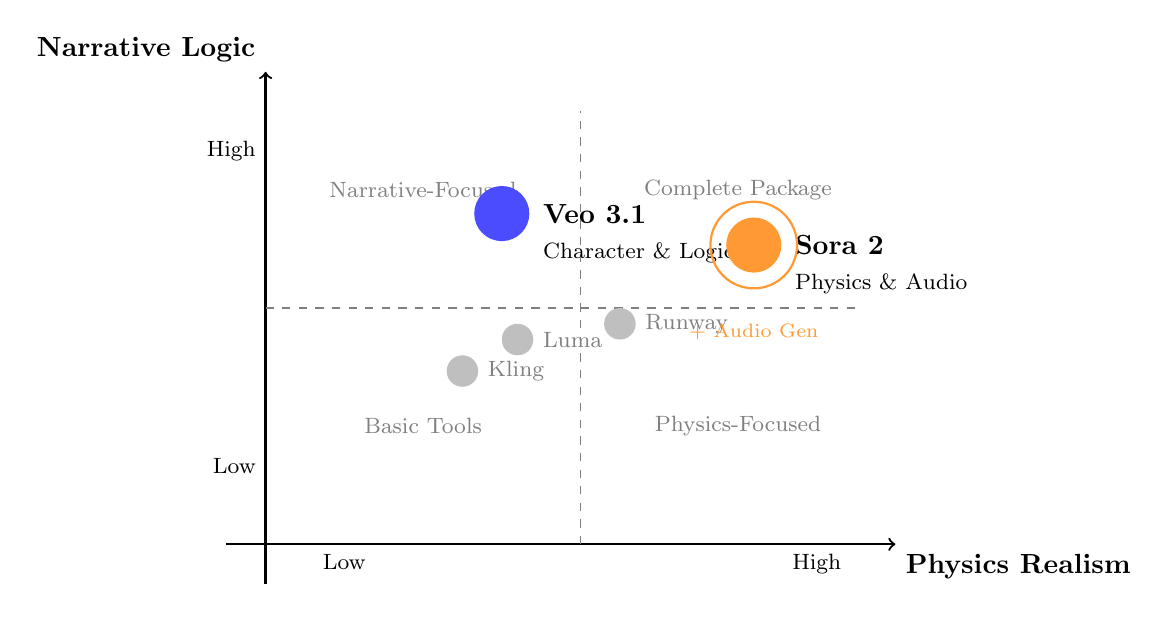
\begin{tikzpicture}[scale=1.0]
    % Draw axes
    \draw[thick,->] (-0.5,0) -- (8,0) node[anchor=north west] {\textbf{Physics Realism}};
    \draw[thick,->] (0,-0.5) -- (0,6) node[anchor=south east] {\textbf{Narrative Logic}};

    % Axis labels
    \node at (1,0) [below] {\footnotesize Low};
    \node at (7,0) [below] {\footnotesize High};
    \node at (0,1) [left] {\footnotesize Low};
    \node at (0,5) [left] {\footnotesize High};

    % Quadrant labels (light gray background)
    \node at (2,4.5) [text=gray] {\footnotesize Narrative-Focused};
    \node at (6,4.5) [text=gray] {\footnotesize Complete Package};
    \node at (2,1.5) [text=gray] {\footnotesize Basic Tools};
    \node at (6,1.5) [text=gray] {\footnotesize Physics-Focused};

    % Dashed center lines
    \draw[dashed,gray] (4,0) -- (4,5.5);
    \draw[dashed,gray] (0,3) -- (7.5,3);

    % Veo 3.1 position (high narrative, medium physics)
    \fill[blue!70] (3,4.2) circle (0.35);
    \node[right] at (3.4,4.2) {\textbf{Veo 3.1}};
    \node[right,font=\footnotesize] at (3.4,3.7) {Character \& Logic};

    % Sora 2 position (high physics, medium-high narrative)
    \fill[orange!80] (6.2,3.8) circle (0.35);
    \node[right] at (6.6,3.8) {\textbf{Sora 2}};
    \node[right,font=\footnotesize] at (6.6,3.3) {Physics \& Audio};

    % Other platforms for context (smaller, lighter)
    \fill[gray!50] (2.5,2.2) circle (0.2);
    \node[right,font=\footnotesize,gray] at (2.7,2.2) {Kling};

    \fill[gray!50] (4.5,2.8) circle (0.2);
    \node[right,font=\footnotesize,gray] at (4.7,2.8) {Runway};

    \fill[gray!50] (3.2,2.6) circle (0.2);
    \node[right,font=\footnotesize,gray] at (3.4,2.6) {Luma};

    % Audio capability indicator (Sora 2 unique feature)
    \draw[orange!80,thick] (6.2,3.8) circle (0.55);
    \node[orange!80,font=\scriptsize] at (6.2,2.7) {+ Audio Gen};

\end{tikzpicture}
\caption{Platform Positioning Quadrant: Sora 2 vs.\ Veo 3.1. The orange ring around Sora 2 indicates its unique audio generation capability---a critical differentiator for social media content creators.}
\label{fig:platform-quadrant}
\end{figure}

\begin{resultbox}[Reading the Quadrant]
\textbf{Upper-Right (Ideal Zone):} Both platforms aspire to this quadrant. Sora 2 currently leads in physics with strong narrative; Veo 3.1 leads in narrative with acceptable physics.

\textbf{Key Insight:} The \textcolor{orange}{\textbf{orange ring}} around Sora 2 represents its \textit{exclusive audio generation capability}---neither Veo 3.1 nor any competitor (Runway, Kling, Luma) can match this. For TikTok/Reels creators, this alone may determine your platform choice.
\end{resultbox}

%% ================================================================
\section{Core Methodology: The Five-Dimension Prompt Formula}
\label{sec:five-dimension-formula}

\begin{yellowbox}[Expert Tip: Google's Official Prompt Formula]
Regardless of which model you use, following this structure will dramatically improve generation quality:

\vspace{0.5em}
\centering
\large\textbf{Camera + Subject + Action + Background + Style}
\end{yellowbox}

This formula represents the ``golden rule'' emphasized by Google's official team during the Veo launch. It also serves as the foundational logic for all major AI video models, including Sora, Runway, Kling, and Luma.

\subsection{Why Structure Matters}

When Prompts lack structure, AI models resort to ``guessing.'' The five-dimension formula translates the director's (user's) intent precisely to the AI, transforming random generation into command execution.

\subsection{Dimension 1: Camera --- Defining the Viewer's Perspective}
\label{subsec:dim-camera}

The camera dimension represents the fundamental difference between video and static images. Without explicit camera instructions, AI typically generates a static, surveillance-style viewpoint.

\textbf{Purpose:} Guide visual attention and create cinematic feel.

\paragraph{Movement Types:}
\begin{itemize}
    \item \texttt{Zoom in / Zoom out} --- Push toward or pull away from subject
    \item \texttt{Pan left / Pan right} --- Horizontal camera rotation
    \item \texttt{Tracking shot} --- Camera follows moving subject
    \item \texttt{Orbit / 360-degree arc} --- Camera circles around subject
    \item \texttt{Crane shot} --- Vertical movement up or down
\end{itemize}

\paragraph{Lens Types:}
\begin{itemize}
    \item \texttt{Wide angle} --- Expansive field of view, environmental context
    \item \texttt{Telephoto / Close-up} --- Compressed perspective, intimate detail
    \item \texttt{Macro} --- Extreme close-up for tiny details
    \item \texttt{Drone shot / Aerial view} --- Bird's eye perspective
    \item \texttt{POV (Point of View)} --- First-person perspective
\end{itemize}

\paragraph{Special Effects:}
\begin{itemize}
    \item \texttt{Handheld shaky cam} --- Documentary-style movement
    \item \texttt{Low angle (upward)} --- Subject appears powerful, imposing
    \item \texttt{High angle (downward)} --- Subject appears vulnerable, small
    \item \texttt{Dutch angle} --- Tilted frame for unease or dynamism
\end{itemize}

\subsection{Dimension 2: Subject --- Establishing the Visual Center}
\label{subsec:dim-subject}

The more specific your subject description, the less likely the AI will produce ``hallucinations.'' Never write simply ``a person''---describe their characteristics in detail.

\textbf{Purpose:} Establish visual focus and maintain character consistency.

\paragraph{Physical Attributes:}
\begin{itemize}
    \item Age, ethnicity, build, distinctive features
    \item Skin texture (weathered face, freckles, wrinkles)
    \item Hair style, color, and condition
\end{itemize}

\paragraph{Clothing and Accessories:}
\begin{itemize}
    \item Material (silk, denim, leather, wool)
    \item Color and pattern specifics
    \item Style period (vintage, cyberpunk, formal, casual)
\end{itemize}

\paragraph{Object Details:}
\begin{itemize}
    \item For vehicles: make, model, color, condition (scratches, dust)
    \item For food: texture, steam, moisture, freshness indicators
    \item For products: brand elements, material finish, wear patterns
\end{itemize}

\subsection{Dimension 3: Action --- Bringing the Scene to Life}
\label{subsec:dim-action}

Action is what makes video \textit{video}. Static descriptions (``a person standing'') produce mere animated photographs---PowerPoint slides with movement. Describe continuous, evolving action.

\textbf{Purpose:} Infuse vitality and demonstrate physical laws.

\paragraph{Explicit Behaviors:}
\begin{itemize}
    \item Running, dancing, drinking, laughing, turning to look, typing
    \item Interacting with objects: picking up, putting down, throwing, catching
\end{itemize}

\paragraph{Physical States:}
\begin{itemize}
    \item Explosion, shattering, melting, flowing, pouring
    \item Smoke billowing, wind blowing through hair, rain falling
\end{itemize}

\paragraph{Micro-actions (Reality Enhancement):}
\begin{itemize}
    \item Blinking, sighing, fingers tapping on desk
    \item Adjusting tie, brushing hair aside, subtle weight shifts
\end{itemize}

\subsection{Dimension 4: Background --- Environment and Atmosphere}
\label{subsec:dim-background}

Background encompasses more than location---it includes lighting and temporal context. These elements establish the overall mood and narrative framework.

\textbf{Purpose:} Provide narrative context and enhance immersion.

\paragraph{Location Types:}
\begin{itemize}
    \item Cyberpunk street, minimalist white room, dense rainforest
    \item Abandoned factory, luxury penthouse, crowded marketplace
    \item Abstract void, infinite gradient, studio backdrop
\end{itemize}

\paragraph{Lighting (Critical Element):}
\begin{itemize}
    \item \texttt{Golden hour} --- Warm, directional sunset/sunrise light
    \item \texttt{High noon} --- Harsh overhead sunlight, strong shadows
    \item \texttt{Neon lighting} --- Colorful artificial urban illumination
    \item \texttt{Window light} --- Soft, diffused natural indoor lighting
    \item \texttt{Rembrandt lighting} --- Classic portrait lighting with shadow triangle
    \item \texttt{Volumetric lighting / God rays} --- Visible light beams through atmosphere
\end{itemize}

\paragraph{Weather Conditions:}
\begin{itemize}
    \item Heavy rain, thick fog, falling snow, sandstorm
    \item Clear sky, overcast, dramatic storm clouds
    \item Mist, haze, dust particles in light
\end{itemize}

\subsection{Dimension 5: Style --- The Art Director's Vision}
\label{subsec:dim-style}

Style defines the visual ``texture'' of your output. Is it an animated cartoon or a Hollywood blockbuster?

\textbf{Purpose:} Unify visual aesthetics and establish quality ceiling.

\paragraph{Medium:}
\begin{itemize}
    \item \texttt{35mm film} --- Classic cinema grain and color science
    \item \texttt{VHS aesthetic} --- Retro video tape artifacts
    \item \texttt{Unreal Engine 5 / 3D render} --- Photorealistic CGI look
    \item \texttt{Anime / Japanese animation} --- Stylized 2D animation
    \item \texttt{Oil painting style} --- Painterly, artistic interpretation
\end{itemize}

\paragraph{Quality Specifications:}
\begin{itemize}
    \item Resolution: 4K, 8K, cinematic resolution
    \item Detail level: highly detailed, intricate, photorealistic
    \item Render quality: ray-traced, physically accurate, studio quality
\end{itemize}

\paragraph{Aesthetic Movements:}
\begin{itemize}
    \item \texttt{Film noir} --- High contrast black and white, dramatic shadows
    \item \texttt{Vaporwave} --- Retro-futuristic, pink/cyan palette, 80s nostalgia
    \item \texttt{Minimalist} --- Clean, simple, essential elements only
    \item \texttt{Baroque} --- Ornate, dramatic, rich detail
    \item \texttt{Documentary} --- Authentic, unpolished, observational
\end{itemize}

%% ================================================================
\section{Practical Application: Before and After}
\label{sec:before-after}

To illustrate the transformative power of structured prompting, consider the following comparison:

\subsection{Unstructured Prompt (Ineffective)}

\begin{warnbox}[$\times$ Poor Prompt Example]
\texttt{"A cat eating something."}
\end{warnbox}

\textbf{Typical Result:} The AI generates a cat rigidly facing the camera, mouth mechanically moving, background undefined and blurry. No aesthetic appeal, no narrative, no cinematic quality.

\subsection{Structured Prompt (Effective)}

\begin{resultbox}[$\checkmark$ Optimized Prompt Using Five-Dimension Formula]
\small
\textbf{(Camera)} Low-angle close-up shot, focused on the cat's face $\rightarrow$ \textbf{(Subject)} A fluffy orange tabby cat with clearly visible whiskers $\rightarrow$ \textbf{(Action)} Enthusiastically chewing a bowl of wet cat food, occasionally licking its lips with satisfaction $\rightarrow$ \textbf{(Background)} Sunlit modern kitchen floor, background softly blurred with morning light streaming across the tiles $\rightarrow$ \textbf{(Style)} 4K quality, National Geographic documentary style, realistic fur texture.
\end{resultbox}

\textbf{Expected Result:} A cinematic, emotionally engaging clip with professional composition, natural behavior, and broadcast-quality production values.

%% ================================================================
\section{Professional Tips for Optimal Results}
\label{sec:pro-tips}

\begin{tipbox}[Pro Tip \#1: Prompt Order Matters]
AI models typically assign highest weight to information at the beginning of Prompts. Place your most critical elements---\textbf{Subject} and \textbf{Camera}---at the front of your Prompt for maximum influence on the output.
\end{tipbox}

\begin{tipbox}[Pro Tip \#2: Adjectives Are Your Seasoning]
Even with identical formula structure, ``\textit{angry} movement'' and ``\textit{graceful} movement'' produce dramatically different videos. Invest time in selecting expressive, evocative adjectives that convey the precise emotional tone you envision.
\end{tipbox}

\begin{tipbox}[Pro Tip \#3: Platform-Specific Optimization]
Based on our evaluation findings:
\begin{itemize}
    \item \textbf{For Sora 2:} Emphasize complex \textbf{Action} descriptions. Sora's physics engine can handle sophisticated movement instructions that would confuse other models.
    \item \textbf{For Veo 3.1:} Focus on \textbf{Camera} and \textbf{Style} dimensions. Veo excels at interpreting artistic and cinematographic language, producing stable, aesthetically coherent results.
\end{itemize}
\end{tipbox}

\begin{tipbox}[Pro Tip \#4: Iterative Refinement]
Neither platform produces perfect results on the first attempt. Adopt an iterative workflow:
\begin{enumerate}
    \item Generate initial output with complete five-dimension Prompt
    \item Identify specific deficiencies (physics, consistency, detail)
    \item Adjust relevant dimensions and regenerate
    \item Repeat until satisfactory results achieved
\end{enumerate}
\end{tipbox}

%% ================================================================
\section{Chapter Summary: The Enduring Framework}
\label{sec:chapter-summary}

This chapter provided more than a platform comparison---it established a \textbf{reusable evaluation framework} that you can apply to any AI video generation tool, present or future. Let us distinguish between what is temporary and what is permanent:

\subsection*{What Will Change (Platform-Specific Results)}

The specific findings below reflect late 2025 capabilities and \textit{will} become outdated:

\begin{enumerate}
    \item \textbf{Current Standings:} Veo 3.1 and Sora 2 excel in different domains. Platform selection should be driven by project requirements, not brand preference.

    \item \textbf{Veo 3.1 Strengths (as of late 2025):} Temporal consistency, anatomical stability, logical coherence, and emotional expression.

    \item \textbf{Sora 2 Strengths (as of late 2025):} Physics simulation, material rendering, cinematography, and audio integration.

    \item \textbf{Audio Generation Status:} As of late 2025, Sora 2 remains the only platform with native synchronized audio generation.
\end{enumerate}

\subsection*{What Will Endure (The Methodology)}

These principles will remain valuable regardless of which platforms dominate:

\begin{enumerate}
    \item \textbf{The Five-Dimension Evaluation Framework:} Test any new platform across temporal evolution, physics simulation, emotional expression, hand-object interaction, and commercial readiness. This systematic approach reveals true capabilities beyond marketing claims.

    \item \textbf{The Five-Dimension Prompt Formula:} Camera + Subject + Action + Background + Style. This structure works across all major AI video platforms and will continue to work as models evolve.

    \item \textbf{Platform-Specific Optimization:} Every platform has architectural biases. Learning to identify and leverage these biases is a transferable skill.

    \item \textbf{The Evaluation Mindset:} Don't ask ``Which is best?'' Ask ``Which is best \textit{for this specific task}?'' Then design tests to answer that question empirically.
\end{enumerate}

\begin{resultbox}[The Bottom Line: Methodology Over Rankings]
\textbf{When Sora 3 or Veo 4 launches}, don't wait for reviews---run these five test cases yourself. The evaluation framework in this chapter will tell you exactly where the new platform excels and where it falls short.

\textbf{The creators who thrive} in the AI era are not those who memorize which tool is ``best,'' but those who can rapidly evaluate any new tool and integrate it into their workflow.
\end{resultbox}

\begin{quote}
\textit{\textbf{Timeless Principle:} Platforms evolve, interfaces change, and today's leader may be tomorrow's legacy system. But the underlying visual logic---light, composition, rhythm, physics, and emotional resonance---remains eternal. Master these fundamentals, and you will adapt effortlessly to any future tool.}
\end{quote}

As both platforms continue rapid development, these relative strengths may shift. However, the fundamental principle remains constant: \textit{understanding your creative requirements and systematically matching them to platform capabilities is the key to successful AI video generation}.


